\section{Probabilistic programming with programmable inference in GenLite}

\begin{figure}[t]
\centering
    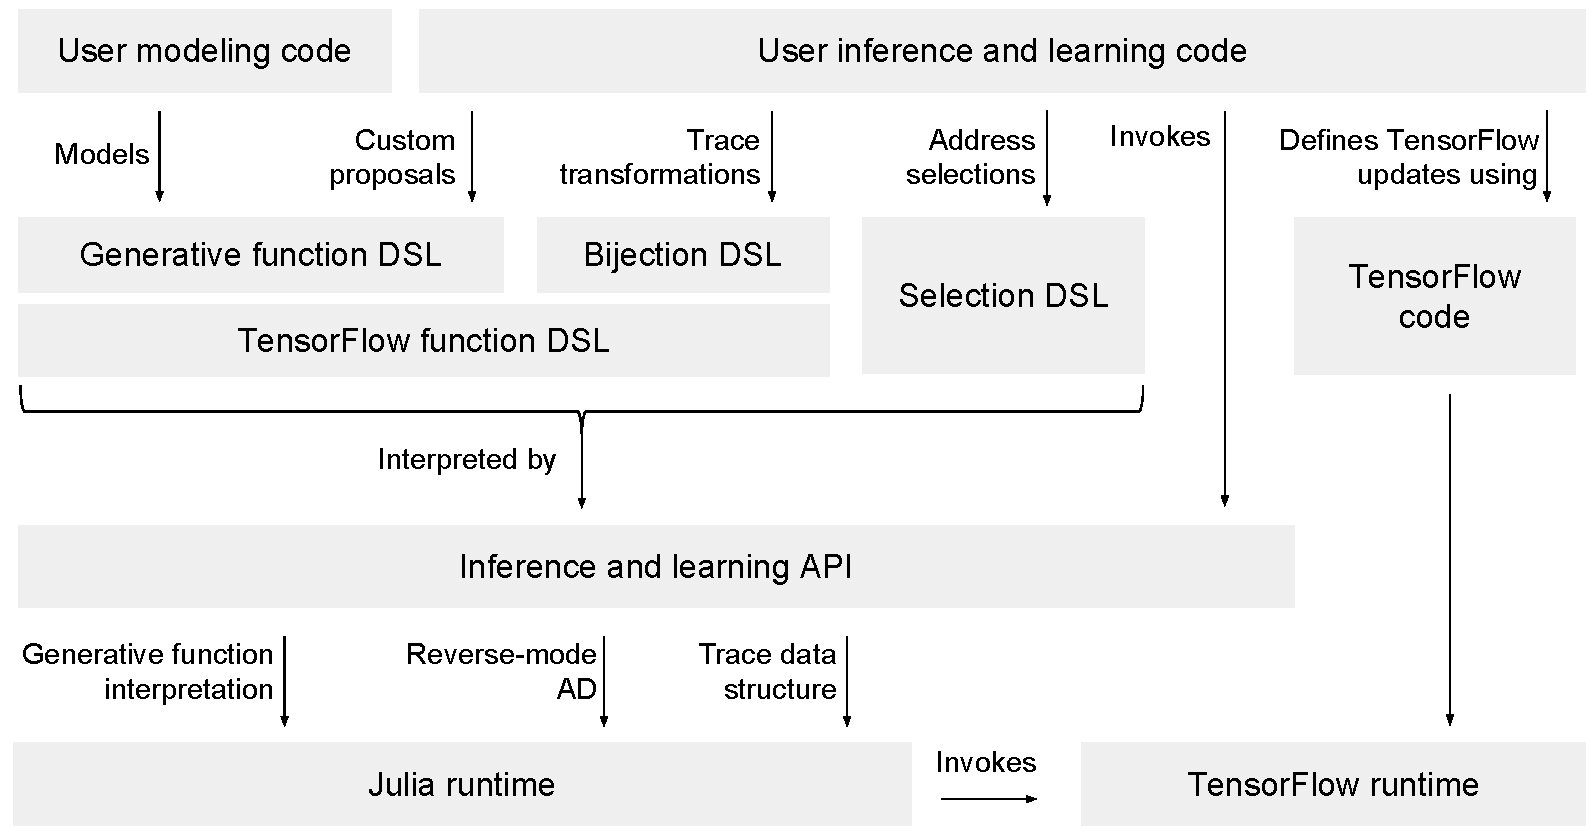
\includegraphics[width=\textwidth]{images/genlite-schematic.pdf}
    \caption{Architecture of GenLite including the TensorFlow extention}
    \label{fig:genlite-schematic}
\end{figure}

GenLite is a probabilistic modeling and inference platform implemented on top of Julia \cite{TODO}.
GenLite consists of a probabilistic programming language embedded in Julia, and an inference and learning API.
Users define generative models by writing \emph{generative functions}, which are Julia functions that are augmented with random choices that play the role of latent and observed random variables.
Unlike other probabilistic programming platforms, users implement inference algorithms in host language (Julia) code, building on high-level abstractions provided by the inference and learning API.
GenLite also contains auxiliary domain-specific languages for inference, which augment Julia functions with additional behavior and semantics:
First, \emph{selection functions} are used to identify subsets of random choices, and \emph{bijective functions} are used to define probability-preserving transformations between latent variable representations.
The remainder of this section describes the subset of features of GenLite that are necessary for user-programmable inference based on deep learning.

\subsection{Generative function DSL}

A generative function is a Julia function annotated with $\gengen{}$.
A generative function behaves like a regular Julia function, except that it is functional with respect to its arguments (i.e. it should not mutate its arguments or any global state), and it has access to additional probabilistic language constructs.
Together these properties allow it to represent a probability distribution.
This section describes the additional language constructs.

\paragraph{Random choices and traces}
First, generative functions can make random choices (i.e. sample random values).
Random choices are typically drawn according to built-in or user-specified probability distributions.
For example the expression $\code{normal(mu, sig)}$ evaluates to a random draw from a normal distribution with mean $\code{mu}$ and standard-deviation $\code{std}$.
A random choice is typically assigned an \emph{address}, using the syntax $\code{@addr(normal(mu, std), addr)}$, where $\code{addr}$ is a dynamically computed string, or tuple of strings (which denote a hierarchical address).
Within every possible execution of the program, the random choices must have unique addresses.
Assuming that a generative function terminates (i.e. returns) with probability one\footnote{Verifying termination with probability one for arbitrary functions embeds the halting problem}, a generative function defines a probability distribution on \emph{traces}, which are associative collections that map the address of a random choice to its value.
In the simple setting where the set of addresses that are sampled is constant across all executions, the GenLite function denotes a joint distribution on a collection of random variables identified with addresses.
A formal semantics for GenLite generative functions is outside the scope of this paper.
Informally, the probability of a certain trace is the product of the probability that each address was assigned its given value in the trace, if the trace is the result of some possible execution of the program, and zero otherwise.
We denote the probability of a trace $t$ for generative function $p$ by $p(t)$.
When continuous random choices are included, a generative function that terminates with probability one denotes a probability measure on traces.
See \cite{CusumanoPLDI2018} and \cite{Borgstrom} for examples of trace-based semantics for probabilistic programming languages.
Finally, note that not all random choices made by a generative function need to be assigned addresses---random choices without addresses are called \emph{untraced}.
The ability to make untraced random choices means that GenLite functions can invoke arbitrary black box code.

\paragraph{Reading from an input trace}
Each generative function defines a distribution on its own trace.
In addition, a generative function may optionally read from an \emph{input trace}, using the syntax $\code{@read(addr)}$, where $\code{addr}$ is a dynamically computed string or tuple of strings.
As will be discussed in more detail below, input traces enable generative functions to be used to define proposal distribution in Markov chain Monte Carlo (MCMC) and importance sampling and sequential Monte Carlo inference algorithms.

\paragraph{Trainable static parameters}
Generative functions can also contain \emph{trainable static parameters}.
These parameters are declared at the beginning of the generative function definition using the syntax $\code{@param name}$ or, with an optional type declaration: $\code{@param name::type}$.
These parameters are static in the sense that all invocation of the generative function make use of the same values for these parameters.
The values of static parameters are set by the user in Julia code, using the API method $\code{set\_param!(gf, name, value)}$, where $\code{gf}$ is a reference to the generative function.
Gradients with respect to static parameters are obtained by the user with $\code{get\_param\_grad(gf, name)}$.
Gradients are discussed in more detail below in the section on training generative functions (Section~\ref{sec:training}).

\paragraph{Calling other generative functions}
Finally, generative functions can invoke other generative functions, in three ways:
First, a generative function may make an \emph{untraced invocation}, using regular function invocation syntax (e.g. $\code{fn(args..)}$).
Second, a generative function may invoke a generative function using the syntax $\code{@addr(fn(args...), addr)}$, which indicates that the entire trace of the function $\code{fn}$ should be placed in a sub-trace of the current function's trace, under namespace $\code{addr}$.
Third, a generative function may use $\code{@splice(fn(args...))}$, which indicates that the trace of $\code{fn}$ should be spliced into the current trace, without introducing a separate namespace.
It is an error if any addresses in the trace of $\code{fn}$ collide with any address assigned by the caller.
The use of $\code{@addr}$ to make random choices, combined with its use to invoke other generative functions, means that the trace of a generative function is in general a hierarchical data structure.

\subsection{Selection function DSL}
A \emph{selection function} is a Julia function annotated with $\code{@selection}$.
Users write selection functions to define sets of addresses within a trace, called \emph{selections}.
These selections can be used to identify which random choices should be re-proposed by the $\code{mh}$ operator (see below) or which random choices should be targeted for MAP estimtaion by the $\code{map\_optimize}$ operator (see below).
Selection functions can invoke the $\code{@select(addr)}$ construct, which indicates that the address $\code{addr}$ should be added to the selection, where $\code{addr}$ is a string or tuple of strings.
Selection functions can also invoke a selection function $\code{fn}$ using either $\code{@addr(fn(args..), addr)}$ (which sets the namespace of the callee to $\code{addr}$) or $\code{@splice(fn(args..))}$.
Finally, selection functions can read from the trace whose addresses they are selecting using $\code{@read(addr)}$.

\subsection{Bijection function DSL}
A \emph{bijection function} is a Julia function annotated with $\code{@bijection}$.
Users write bijection functions to define invertible (deterministic) transformations between sets of traces.
Bijection functions are applied in the context of an \emph{input trace} and an \emph{output trace}.
The bijection function reads from the input trace using $\code{@read(addr)}$ and writes to the output trace using $\code{@write(value, addr)}$.
Additional convenience functions include $\code{@copy(inaddr, outaddr)}$, which is an alias for a $\code{@read}$ followed by a $\code{@write}$, and $\code{@copyall(inaddr, outaddr)}$, which copies the sub-trace of the input trace rooted at $\code{inaddr}$ to the sub-trace of the output trace rooted at $\code{outaddr}$.
Similar to generative functions and selection functions, bijection functions can invoke other bijection functions using $\code{@addr(fn(args..), addr)}$ and $\code{@splice(fn(args..))}$.
When a bijection function reads and writes continuous random choices, the GenLite runtime computes the Jacobian of the transformation from the input trace to the output trace using reverse-mode automatic differentiation.
The Jacobian can be used to compute the probability density of the output trace, given the probability density of the input trace.
Bijection functions are used to rearrange addresses in traces, as well as to define change-of-variable transformations used in e.g. reversible-jump MCMC \cite{Green1994}.

\subsection{High-level embedded inference programming}

\begin{figure}[t]
\centering
    \includegraphics[width=\textwidth]{images/gen-api.pdf}
    \caption{GenLite inference and learning API (shaded boxes denote methods)}
    \label{fig:genlite-api}
\end{figure}

In GenLite, users implement inference and learning algorithms in Julia, using an inference and learning API provided by GenLite (Figure~\ref{fig:genlite-api}).
The API provides a variety of methods that are parametrized by generative functions, selection functions, and/or bijection functions.
Because inference and learning algorithms are implemented in Julia, users can make use of Julia's existing abstractions (e.g. for loops, procedural abstraction), usability features (e.g. error messages, profiler), package ecosystem, and foreign interfaces to compose inference algorithms.

\paragraph{Traces are user-space values.} Most of these methods either consume or produce traces of generative functions, which are user-space Julia values of type $\code{Trace}$.
A $\code{Trace}$ is a hierarchical data structure resembling a trie that stores values of random choices at hierarchical addresses.
Users encode observed values of random choices by constructing a $\code{Trace}$ containing just values for the observed random choices, called an \emph{observation trace}.
The GenLite inference and learning API contains a number of methods for implementing inference and learning algorithms involving generative models.
The full set of methods, which includes support for sequential Monte Carlo, reversible-jump MCMC, and user-defined auxiliary-variable algorithms, is outside the scope of this paper.
Instead, we describe a subset of API methods that are relevant for user-programmable deep learning for inference.

\paragraph{Sampling from a generative funtion with $\code{simulate}$.}
The simplest operation we can perform with a generative function is to execute it.
The $\code{simulate}$ method takes a generative function and its arguments (and an optional input trace not shown), and executes it, and returns the trace of the execution, the return value of the function, and the log probability of the trace, which we refer to from here onwards as the `score':
\begin{verbatim}
(trace::Trace, score::Float64, val) = simulate(fn::GenFunction, args::Tuple)
\end{verbatim}

\paragraph{Importance sampling using $\code{imp}$.}
The simplest inference operation is importance sampling using the prior as the proposal, which is implemented by the method $\code{imp}$.
The method takes a generative function that represents the generative model and its arguments, as well as an observation trace.
The method returns a trace that includes the given observations, as well as newly sampled latent random choices, which are sampled using forward simulation (i.e. the prior).
The method also returns the score of the resulting trace, the log importance weight, and the return value of the model function.
\begin{verbatim}
(trace::Trace, score::Trace, log_weight, val) = imp(
        model::GenFunction, args::Tuple, observations::Trace)
\end{verbatim}
Note that this method does not run an importance-sampling algorithm per se because it does not generate multiple importance samples, normalize their weights, or resample.
Instead, these operations are implemented in user code using regular Julia abstractions.

\paragraph{Importance sampling with a custom proposal using $\code{imp2}$.}
It is also possible to perform importance sampling using user-defined proposal distributions that are specified as generative functions.
\begin{verbatim}
(trace::Trace, score::Float64, log_weight::Float64, val) = imp2(
    model::GenFunction, model_args::Tuple,
    proposal::GenFuntion, proposal_args::Tuple, 
    observations::Trace)
\end{verbatim}
The addresses of the latent traced random choices in the model function must match exactly with the addresses of the traced random choices in the proposal.
Because proposals are defined as general probabilistic programs, they can include standard distributions, deep neural networks (see Section~\ref{sec:TODO}) and algorithmic proposals as discussed in \cite{Cusumano2016}.

\paragraph{Resimulation Metropolis-Hastings with $\code{mh}$.}
% TODO

\paragraph{Metropolis-Hastings with a custom proposal with $\code{mh2}$.}
% TODO

\paragraph{Training generative functions using $\genbackprop{}$.} \label{sec:training}
% TODO
A building block that is used for training the static parameters of generative functions is \texttt{backprop}, which has the following type signature:
\begin{center}
    \texttt{backprop(fn::GenerativeFunction, args::Tuple, trace::Trace, [input\_trace::Trace])}
\end{center}
The trace must be a complete trace of the given generative function for the given arguments to the function.
This method computes the gradient of the log probability of the trace with respect to all static parameters, using reverse-mode automatic differentiation (AD).
Each static parameter has a \emph{gradient accumulator}, which is a value that is incremented by the gradient during each call to \texttt{backprop}.
User Julia code reads and write to the gradient accumulator values and the values of static parameters to perform parameter updates, using GenLite methods:\\
\texttt{set\_param!(fn::GenerativeFunction, name::Symbol, value)}\\
\texttt{get\_param(fn::GenerativeFunction, name::Symbol)}\\
\texttt{get\_param\_grad(fn::GenerativeFunction, name::Symbol)}\\
\texttt{zero\_param\_grad!(fn::GenerativeFunction, name::Symbol)}

\paragraph{Gradient-based MAP using $\gentracegrad{}$.}
% TODO
